\documentclass[11pt,a4paper]{report}
\usepackage[textwidth=37em,vmargin=30mm]{geometry}
\usepackage{calc,xunicode,amsmath,amssymb,paralist,enumitem,tabu,booktabs,datetime2,xeCJK,xeCJKfntef,listings}
\usepackage{tocloft,fancyhdr,tcolorbox,xcolor,graphicx,eso-pic,xltxtra,xelatexemoji}

\newcommand{\envyear}[0]{2025}
\newcommand{\envdatestr}[0]{2025-05-29}
\newcommand{\envfinaldir}[0]{webdb/2025/20250529/final}

\usepackage[hidelinks]{hyperref}
\hypersetup{
    colorlinks=false,
    pdfpagemode=FullScreen,
    pdftitle={Web Digest - \envdatestr}
}

\setlength{\cftbeforechapskip}{10pt}
\renewcommand{\cftchapfont}{\rmfamily\bfseries\large\raggedright}
\setlength{\cftbeforesecskip}{2pt}
\renewcommand{\cftsecfont}{\sffamily\small\raggedright}

\setdefaultleftmargin{2em}{2em}{1em}{1em}{1em}{1em}

\usepackage{xeCJK,xeCJKfntef}
\xeCJKsetup{PunctStyle=plain,RubberPunctSkip=false,CJKglue=\strut\hskip 0pt plus 0.1em minus 0.05em,CJKecglue=\strut\hskip 0.22em plus 0.2em}
\XeTeXlinebreaklocale "zh"
\XeTeXlinebreakskip = 0pt


\setmainfont{Brygada 1918}
\setromanfont{Brygada 1918}
\setsansfont{IBM Plex Sans}
\setmonofont{JetBrains Mono NL}
\setCJKmainfont{Noto Serif CJK SC}
\setCJKromanfont{Noto Serif CJK SC}
\setCJKsansfont{Noto Sans CJK SC}
\setCJKmonofont{Noto Sans CJK SC}

\setlength{\parindent}{0pt}
\setlength{\parskip}{8pt}
\linespread{1.15}

\lstset{
	basicstyle=\ttfamily\footnotesize,
	numbersep=5pt,
	backgroundcolor=\color{black!5},
	showspaces=false,
	showstringspaces=false,
	showtabs=false,
	tabsize=2,
	captionpos=b,
	breaklines=true,
	breakatwhitespace=true,
	breakautoindent=true,
	linewidth=\textwidth
}






\newcommand{\coverpic}[2]{
    % argv: itemurl, authorname
    Cover photo by #2~~(\href{#1}{#1})
}
\newcommand{\makeheader}[0]{
    \begin{titlepage}
        % \newgeometry{hmargin=15mm,tmargin=21mm,bmargin=12mm}
        \begin{center}
            
            \rmfamily\scshape
            \fontspec{BaskervilleF}
            \fontspec{Old Standard}
            \fontsize{59pt}{70pt}\selectfont
            WEB\hfill DIGEST
            
            \vfill
            % \vskip 30pt
            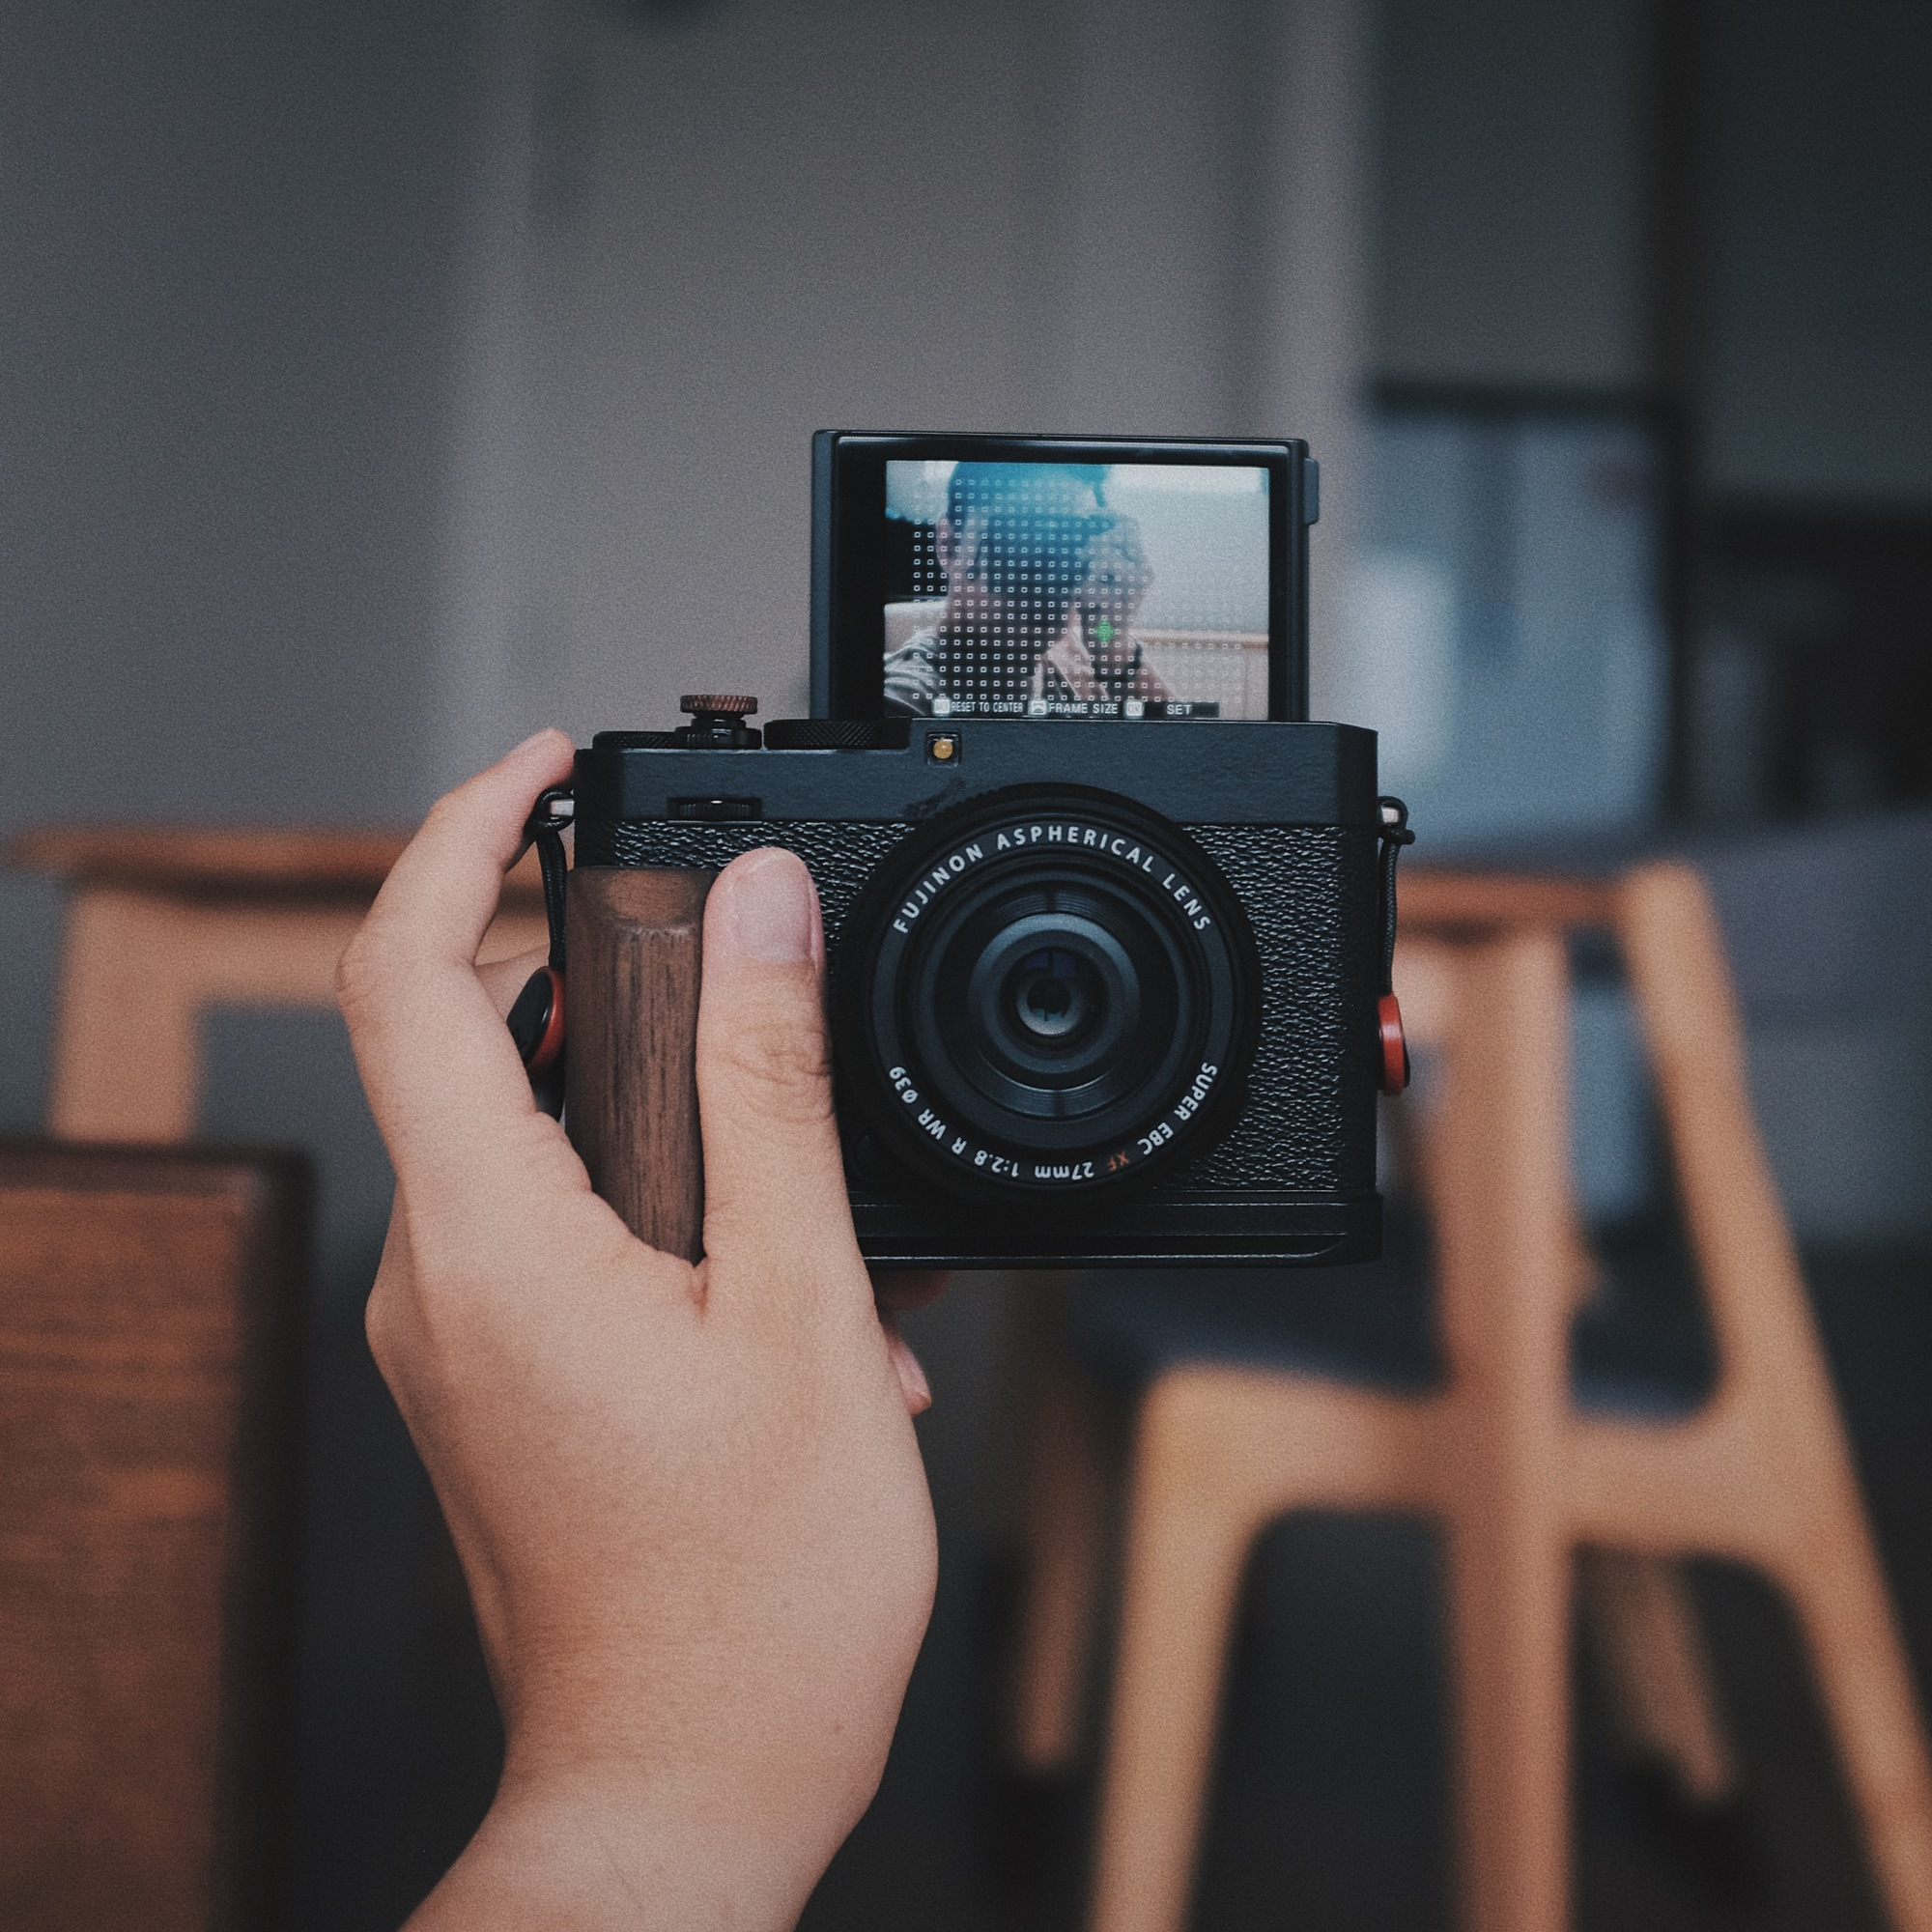
\includegraphics[width=\linewidth]{\envfinaldir/coverpic-prod.jpg}\par
            % \vskip 30pt
            \vfill

            \normalsize\rmfamily\scshape
            \copyright{} The Web Digest Project \hfill\large \envdatestr
        \end{center}
    \end{titlepage}
    % \restoregeometry
}
\newcommand{\simplehref}[1]{%
    \textcolor{blue!80!green}{\href{#1}{#1}}%
}
\renewcommand{\contentsname}{\center\Huge\sffamily\bfseries Contents\par\vskip 20pt}
\newcounter{ipartcounter}
\setcounter{ipartcounter}{0}
\newcommand{\ipart}[1]{
    % \vskip 20pt
    \clearpage
    \stepcounter{ipartcounter}
    \phantomsection
    \addcontentsline{toc}{chapter}{#1}
    % \begin{center}
    %     \Huge
    %     \sffamily\bfseries
    %     #1
    % \end{center}
    % \vskip 20pt plus 7pt
}
\newcounter{ichaptercounter}
\setcounter{ichaptercounter}{0}
\newcommand{\ichapter}[1]{
    % \vskip 20pt
    \clearpage
    \stepcounter{ichaptercounter}
    \phantomsection
    \addcontentsline{toc}{section}{\numberline{\arabic{ichaptercounter}}#1}
    \begin{center}
        \Huge
        \sffamily\bfseries
        #1
    \end{center}
    \vskip 20pt plus 7pt
}
\newcommand{\entrytitlefont}[1]{\subsection*{\raggedright\Large\sffamily\bfseries#1}}
\newcommand{\entryitemGeneric}[2]{
    % argv: title, url
    \parbox{\linewidth}{
        \entrytitlefont{#1}\par\vskip 5pt
        \footnotesize\ttfamily\mdseries
        \simplehref{#2}
    }\vskip 11pt plus 11pt minus 1pt
}
\newcommand{\entryitemGithub}[3]{
    % argv: title, url, desc
    \parbox{\linewidth}{
        \entrytitlefont{#1}\par\vskip 5pt
        \footnotesize\ttfamily\mdseries
        \simplehref{#2}\par\vskip 5pt
        \small\rmfamily\mdseries#3
    }\vskip 11pt plus 11pt minus 1pt
}
\newcommand{\entryitemAp}[3]{
    % argv: title, url, desc
    \parbox{\linewidth}{
        \entrytitlefont{#1}\par\vskip 5pt
        \footnotesize\ttfamily\mdseries
        \simplehref{#2}\par\vskip 5pt
        \small\rmfamily\mdseries#3
    }\vskip 11pt plus 11pt minus 1pt
}
\newcommand{\entryitemHackernews}[3]{
    % argv: title, hnurl, rawurl
    % \parbox{\linewidth}{
    %     \entrytitlefont{#1}\par\vskip 5pt
    %     \footnotesize\ttfamily\mdseries
    %     \simplehref{#3}\par
    %     \textcolor{black!50}{\href{#2}{#2}}
    % }\vskip 11pt plus 11pt minus 1pt
    \begin{minipage}{\linewidth}
            \entrytitlefont{#1}\par\vskip 5pt
            \footnotesize\ttfamily\mdseries
            \simplehref{#3}\par
            \textcolor{black!50}{\href{#2}{#2}}
    \end{minipage}\par\vskip 11pt plus 11pt minus 1pt
}







\begin{document}

\makeheader

\tableofcontents\clearpage




\ipart{Developers}
\ichapter{Hacker News}
\entryitemTwoLinks{A toy RTOS inside Super Mario Bros. using emulator save states}{https://news.ycombinator.com/item?id=44120241}{https://prettygoodblog.com/p/what-threads-are-part-2}

\entryitemTwoLinks{Deepseek R1-0528}{https://news.ycombinator.com/item?id=44118818}{https://huggingface.co/deepseek-ai/DeepSeek-R1-0528}

\entryitemTwoLinks{Compiling a neural net to C for a speedup}{https://news.ycombinator.com/item?id=44118373}{https://slightknack.dev/blog/difflogic/}

\entryitemTwoLinks{Show HN: I rewrote my Mac Electron app in Rust}{https://news.ycombinator.com/item?id=44118023}{https://desktopdocs.com/?v=2025}

\entryitemTwoLinks{Japan Post launches 'digital address' system}{https://news.ycombinator.com/item?id=44117779}{https://www.japantimes.co.jp/business/2025/05/27/companies/japan-post-digital-address/}

\entryitemTwoLinks{Compiler Explorer and the promise of URLs that last forever}{https://news.ycombinator.com/item?id=44117722}{https://xania.org/202505/compiler-explorer-urls-forever}

\entryitemTwoLinks{Getting a Cease and Desist from Waffle House}{https://news.ycombinator.com/item?id=44117302}{https://www.jack.bio/blog/wafflehouse}

\entryitemTwoLinks{Show HN: Tesseral – Open-Source Auth}{https://news.ycombinator.com/item?id=44117059}{https://github.com/tesseral-labs/tesseral}

\entryitemTwoLinks{xAI to pay telegram \$300M to integrate Grok into the chat app}{https://news.ycombinator.com/item?id=44116862}{https://techcrunch.com/2025/05/28/xai-to-invest-300m-in-telegram-integrate-grok-into-app/}

\entryitemTwoLinks{Mullvad Leta}{https://news.ycombinator.com/item?id=44116503}{https://leta.mullvad.net}

\entryitemTwoLinks{De-anonymization attacks against the privacy coin XMR}{https://news.ycombinator.com/item?id=44116236}{https://monero.forex/is-monero-totally-private-a-comprehensive-analysis-of-de-anonymization-attacks-against-the-privacy-coin/}

\entryitemTwoLinks{The Blowtorch Theory: A new model for structure formation in the universe}{https://news.ycombinator.com/item?id=44115973}{https://theeggandtherock.com/p/the-blowtorch-theory-a-new-model}

\entryitemTwoLinks{The Who Cares Era}{https://news.ycombinator.com/item?id=44115620}{https://dansinker.com/posts/2025-05-23-who-cares/}

\entryitemTwoLinks{AI: Accelerated Incompetence}{https://news.ycombinator.com/item?id=44114631}{https://www.slater.dev/accelerated-incompetence/}

\entryitemTwoLinks{Microsoft is starting to open Windows Update up to any third-party app}{https://news.ycombinator.com/item?id=44114621}{https://www.theverge.com/news/675446/microsoft-windows-update-all-apps-orchestration-platform}

\entryitemTwoLinks{CheerpJ 4.1: Java in the browser, now supporting Java 17 (preview)}{https://news.ycombinator.com/item?id=44114483}{https://labs.leaningtech.com/blog/cheerpj-4.1}

\entryitemTwoLinks{Cory Doctorow on how we lost the internet}{https://news.ycombinator.com/item?id=44113735}{https://lwn.net/SubscriberLink/1021871/4bec46993258f6b7/}

\entryitemTwoLinks{Why are 2025/05/28 and 2025-05-28 different days in JavaScript?}{https://news.ycombinator.com/item?id=44113397}{https://brandondong.github.io/blog/javascript\_dates/}

\entryitemTwoLinks{As a developer, my most important tools are a pen and a notebook}{https://news.ycombinator.com/item?id=44113210}{https://hamatti.org/posts/as-a-developer-my-most-important-tools-are-a-pen-and-a-notebook/}

\entryitemTwoLinks{Show HN: AutoThink – Boosts local LLM performance with adaptive reasoning}{https://news.ycombinator.com/item?id=44112326}{https://news.ycombinator.com/item?id=44112326}\ichapter{Phoronix}
\entryitemGeneric{\hskip 0pt{}VirtualBox 7.2 Beta Brings Windows 11 Arm Support, Source Code On GitHub}{https://www.phoronix.com/news/Oracle-VirtualBox-7.2-Beta}

\entryitemGeneric{\hskip 0pt{}Linux 6.16 GPU Driver Changes Land: NVIDIA Blackwell, Asahi UAPI, Intel Xe Fan Speeds}{https://www.phoronix.com/news/Linux-6.16-Graphics-Drivers}

\entryitemGeneric{\hskip 0pt{}Git 2.50-rc0 Brings New Improvements}{https://www.phoronix.com/news/Git-2.50-rc0}

\entryitemGeneric{\hskip 0pt{}Big Linux Patch Series Shakes Up The Scheduler Code For Anyone With Only One CPU Core}{https://www.phoronix.com/news/Linux-UP-SMP-Scheduler-2025}

\entryitemGeneric{\hskip 0pt{}AVX-512 Performance + Power Efficiency Shines With AMD Strix Halo}{https://www.phoronix.com/review/amd-strix-halo-avx512}

\entryitemGeneric{\hskip 0pt{}Mesa 25.0.7 Delivers A Last Batch Of Fixes To End The Series}{https://www.phoronix.com/news/Mesa-25.0.7-Released}

\entryitemGeneric{\hskip 0pt{}Linux 6.16 Will Be Able To Exit User Mode Faster: 2~11\% Improvement}{https://www.phoronix.com/news/Linux-616-Faster-Exit-User-Mode}

\entryitemGeneric{\hskip 0pt{}Intel Wildcat Lake Audio Support Merged For Linux 6.16}{https://www.phoronix.com/news/Linux-6.16-Sound}

\entryitemGeneric{\hskip 0pt{}Intel Releases Updated Battlemage Driver Preview Support For Ubuntu 24.04 LTS}{https://www.phoronix.com/news/Ubuntu-24.04-Intel-Preview-1.1}\ichapter{Dribbble}
\entryitemGeneric{\hskip 0pt{}Heyo Turns 2!}{https://dribbble.com/shots/26078572-Heyo-Turns-2}

\entryitemGeneric{\hskip 0pt{}Roaring Bear}{https://dribbble.com/shots/26077332-Roaring-Bear}

\entryitemGeneric{\hskip 0pt{}Smart Home App}{https://dribbble.com/shots/26076565-Smart-Home-App}

\entryitemGeneric{\hskip 0pt{}Fox Brand Mascot}{https://dribbble.com/shots/26077954-Fox-Brand-Mascot}

\entryitemGeneric{\hskip 0pt{}Europe Logo Concept}{https://dribbble.com/shots/26077297-Europe-Logo-Concept}

\entryitemGeneric{\hskip 0pt{}HYDRO - Logo Design}{https://dribbble.com/shots/26073470-HYDRO-Logo-Design}

\entryitemGeneric{\hskip 0pt{}Credit payment card bank app animation}{https://dribbble.com/shots/26063214-Credit-payment-card-bank-app-animation}

\entryitemGeneric{\hskip 0pt{}Kloak Wordmark}{https://dribbble.com/shots/26073220-Kloak-Wordmark}

\entryitemGeneric{\hskip 0pt{}Project Management Dashboard}{https://dribbble.com/shots/26070177-Project-Management-Dashboard}

\entryitemGeneric{\hskip 0pt{}Perception web design}{https://dribbble.com/shots/25995935-Perception-web-design}

\entryitemGeneric{\hskip 0pt{}Stanley // Website}{https://dribbble.com/shots/26056691-Stanley-Website}

\entryitemGeneric{\hskip 0pt{}i SEA you}{https://dribbble.com/shots/26062936-i-SEA-you}

\entryitemGeneric{\hskip 0pt{}AltSocial}{https://dribbble.com/shots/26060858-AltSocial}

\entryitemGeneric{\hskip 0pt{}Fariland Headwear Symbol}{https://dribbble.com/shots/26063219-Fariland-Headwear-Symbol}

\entryitemGeneric{\hskip 0pt{}Animals illustration}{https://dribbble.com/shots/26037153-Animals-illustration}

\entryitemGeneric{\hskip 0pt{}Glassmorphic 3D Logo Animation}{https://dribbble.com/shots/26061835-Glassmorphic-3D-Logo-Animation}

\entryitemGeneric{\hskip 0pt{}Mobile App UI — HR \& Hiring Platform Design}{https://dribbble.com/shots/26061833-Mobile-App-UI-HR-Hiring-Platform-Design}

\entryitemGeneric{\hskip 0pt{}Meditation App Branding Concept}{https://dribbble.com/shots/26057810-Meditation-App-Branding-Concept}

\entryitemGeneric{\hskip 0pt{}Landing Page for an AI-Powered Design System}{https://dribbble.com/shots/26057663-Landing-Page-for-an-AI-Powered-Design-System}

\entryitemGeneric{\hskip 0pt{}Medic H - Logo Design}{https://dribbble.com/shots/26057472-Medic-H-Logo-Design}

\entryitemGeneric{\hskip 0pt{}Smart Home App}{https://dribbble.com/shots/26056748-Smart-Home-App}

\entryitemGeneric{\hskip 0pt{}Fariland Headwear}{https://dribbble.com/shots/26058705-Fariland-Headwear}

\entryitemGeneric{\hskip 0pt{}Sellin dashboard}{https://dribbble.com/shots/26037015-Sellin-dashboard}

\entryitemGeneric{\hskip 0pt{}VE}{https://dribbble.com/shots/26055566-VE}


\ipart{Developers~~~~(zh-Hans)}
\ichapter{Solidot}
\entryitemGeneric{\hskip 0pt{}银河系的一根``骨骼''被脉冲星撞断}{https://www.solidot.org/story?sid=81409}

\entryitemGeneric{\hskip 0pt{}The Browser Company 停止开发 Arc 转向 AI 驱动浏览器 Dia }{https://www.solidot.org/story?sid=81408}

\entryitemGeneric{\hskip 0pt{}AI 模型出现崩溃迹象}{https://www.solidot.org/story?sid=81407}

\entryitemGeneric{\hskip 0pt{}BGP 系统的 Bug 处理方式导致部分网络故障}{https://www.solidot.org/story?sid=81406}

\entryitemGeneric{\hskip 0pt{}鹰利用交通灯捕猎}{https://www.solidot.org/story?sid=81405}

\entryitemGeneric{\hskip 0pt{}腾讯将成为 K-Pop 经纪公司 SM娱乐的第二大股东}{https://www.solidot.org/story?sid=81404}

\entryitemGeneric{\hskip 0pt{}台积电下注基于 MicroLED 的光互联技术}{https://www.solidot.org/story?sid=81403}

\entryitemGeneric{\hskip 0pt{}金星共轨小行星可能威胁到地球}{https://www.solidot.org/story?sid=81402}

\entryitemGeneric{\hskip 0pt{}CIA 曾经秘密运营了一家星球大战粉丝网站}{https://www.solidot.org/story?sid=81401}

\entryitemGeneric{\hskip 0pt{}巴基斯坦分配 2000 MW 电力用于挖掘比特币和 AI 数据中心}{https://www.solidot.org/story?sid=81400}

\entryitemGeneric{\hskip 0pt{}普京表态要封锁微软和 Zoom 的服务}{https://www.solidot.org/story?sid=81399}

\entryitemGeneric{\hskip 0pt{}四名大众前高管因柴油门排放丑闻被判刑}{https://www.solidot.org/story?sid=81398}

\entryitemGeneric{\hskip 0pt{}Firefox 139.0 释出}{https://www.solidot.org/story?sid=81397}

\entryitemGeneric{\hskip 0pt{}新材料被动从空气中收集水分}{https://www.solidot.org/story?sid=81396}

\entryitemGeneric{\hskip 0pt{}SerenityOS 创始人开发自己的独立浏览器 Ladybird}{https://www.solidot.org/story?sid=81395}

\entryitemGeneric{\hskip 0pt{}世界是否需要公有社交网络}{https://www.solidot.org/story?sid=81394}

\entryitemGeneric{\hskip 0pt{}英伟达准备推出新款中国专用 AI 芯片}{https://www.solidot.org/story?sid=81393}

\entryitemGeneric{\hskip 0pt{}木星早期大小是目前的两倍}{https://www.solidot.org/story?sid=81392}

\entryitemGeneric{\hskip 0pt{}天文学家发现黏在一起的双星}{https://www.solidot.org/story?sid=81391}

\entryitemGeneric{\hskip 0pt{}亚马逊程序员感觉他们开始像从事仓库工作的流水线工人}{https://www.solidot.org/story?sid=81390}\ichapter{V2EX}
\entryitemGeneric{\hskip 0pt{}[程序员] 有建站需求的朋友可以看看哈}{https://www.v2ex.com/t/1135036}

\entryitemGeneric{\hskip 0pt{}[问与答] 是否有浏览器扩展可以(或变相)记录到某个页面被删除前的``标签原标题信息''?}{https://www.v2ex.com/t/1135035}

\entryitemGeneric{\hskip 0pt{}[程序员] 在英国做实习开发的一些体验分享}{https://www.v2ex.com/t/1135034}

\entryitemGeneric{\hskip 0pt{}[iOS] 分享 Quantumult X 最小配置}{https://www.v2ex.com/t/1135033}

\entryitemGeneric{\hskip 0pt{}[天黑以后] 20250529 午夜俱乐部}{https://www.v2ex.com/t/1135032}

\entryitemGeneric{\hskip 0pt{}[程序员] TechEmpower 里的一些功能不完善的框架性能数据不具备真实性能意义,造成很多人的误解}{https://www.v2ex.com/t/1135031}

\entryitemGeneric{\hskip 0pt{}[问与答] 域名备案撤销}{https://www.v2ex.com/t/1135030}

\entryitemGeneric{\hskip 0pt{}[Windows] Windows 更新将支持应用更新}{https://www.v2ex.com/t/1135028}

\entryitemGeneric{\hskip 0pt{}[问与答] 老哥们 M4 16+256 5399 和 M3 24+512 6799}{https://www.v2ex.com/t/1135027}

\entryitemGeneric{\hskip 0pt{}[宽带症候群] 移动宽带限制 ipv6 的 pt?}{https://www.v2ex.com/t/1135026}

\entryitemGeneric{\hskip 0pt{}[宽带症候群] 有人使用华为光猫 HN8346Q 联通的吗?支持 IPTV IPoE 模式+用户名密码输入+全路由使能+目的 IP 转发列表吗?}{https://www.v2ex.com/t/1135025}

\entryitemGeneric{\hskip 0pt{}[Google] Google 账号归属地要求越来越严格了?}{https://www.v2ex.com/t/1135023}

\entryitemGeneric{\hskip 0pt{}[程序员] jetbrain 系的 ide 有比较好的 ai 编程解决方案吗?}{https://www.v2ex.com/t/1135022}

\entryitemGeneric{\hskip 0pt{}[分享创造] 告别繁琐的滚动: Prompt Navigator 让 AI 对话历史回溯更轻松!}{https://www.v2ex.com/t/1135021}

\entryitemGeneric{\hskip 0pt{}[程序员] duckdb 太优雅了}{https://www.v2ex.com/t/1135020}

\entryitemGeneric{\hskip 0pt{}[macOS] 垃圾 macos 15.5!}{https://www.v2ex.com/t/1135019}

\entryitemGeneric{\hskip 0pt{}[职场话题] 兄弟们得罪过小人吗?}{https://www.v2ex.com/t/1135018}

\entryitemGeneric{\hskip 0pt{}[问与答] 请问,背调都会问些什么?会卡人吗?}{https://www.v2ex.com/t/1135017}

\entryitemGeneric{\hskip 0pt{}[问与答] 咸鱼网页端客户端怎么老断}{https://www.v2ex.com/t/1135015}

\entryitemGeneric{\hskip 0pt{}[分享创造] 开发了一个 AI 图片生成网站,注册即送免费额度。 如果额度不够, 可以留下邮箱,免费送积分。}{https://www.v2ex.com/t/1135014}

\entryitemGeneric{\hskip 0pt{}[分享创造] [自荐] 无畏契约准星库和生成器}{https://www.v2ex.com/t/1135013}

\entryitemGeneric{\hskip 0pt{}[Java] 请教各位 Java 有没有按照模板从 excel 获取数据的}{https://www.v2ex.com/t/1135011}

\entryitemGeneric{\hskip 0pt{}[职场话题] 裁员赔偿的申请问题}{https://www.v2ex.com/t/1135010}

\entryitemGeneric{\hskip 0pt{}[分享创造] 机器人插件转 MCP,用 QQ 机器人做为 MCP}{https://www.v2ex.com/t/1135008}

\entryitemGeneric{\hskip 0pt{}[Planet] planet 支持 latex 渲染吗}{https://www.v2ex.com/t/1135007}

\entryitemGeneric{\hskip 0pt{}[问与答] 户晨风这个赛道怎么样,这赛道好像只有他一个人,还是蓝海?}{https://www.v2ex.com/t/1135006}

\entryitemGeneric{\hskip 0pt{}[问与答] 如果单纯看吃的,一线城市,哪个更好些?}{https://www.v2ex.com/t/1135005}

\entryitemGeneric{\hskip 0pt{}[程序员] 编程真无聊啊}{https://www.v2ex.com/t/1135004}

\entryitemGeneric{\hskip 0pt{}[投资] 金融数据接口 ig507 官网无法打开,还有推荐吗?}{https://www.v2ex.com/t/1135003}

\entryitemGeneric{\hskip 0pt{}[分享创造] 告别繁琐滚动: Prompt Navigator 让 AI 对话历史回溯更轻松!}{https://www.v2ex.com/t/1135001}

\entryitemGeneric{\hskip 0pt{}[程序员] Gemini 2.5 Pro 05-06 已经封神}{https://www.v2ex.com/t/1135000}

\entryitemGeneric{\hskip 0pt{}[问与答] 为什么显示器要搞窄边框?}{https://www.v2ex.com/t/1134999}

\entryitemGeneric{\hskip 0pt{}[机械键盘] 搭配 macmini 想入一款三模机械键盘, 700 以内}{https://www.v2ex.com/t/1134998}

\entryitemGeneric{\hskip 0pt{}[分享创造] 开发了一款资源导航程序,使用 Nuxt + Go 开发,快速构建资源导航(抽授权码)}{https://www.v2ex.com/t/1134997}

\entryitemGeneric{\hskip 0pt{}[生活] [记录]-2025-05-28 观《猜火车》有感}{https://www.v2ex.com/t/1134996}

\entryitemGeneric{\hskip 0pt{}[问与答] 中国电信,支持按行业订阅营销短信了,你订阅了吗?}{https://www.v2ex.com/t/1134995}

\entryitemGeneric{\hskip 0pt{}[程序员] AI 写 autohotkey 效果不太好}{https://www.v2ex.com/t/1134993}

\entryitemGeneric{\hskip 0pt{}[Apple] 苹果又又又降价了,这次是真心动了}{https://www.v2ex.com/t/1134992}

\entryitemGeneric{\hskip 0pt{}[问与答] 有没有产品经理创业成功的?}{https://www.v2ex.com/t/1134991}

\entryitemGeneric{\hskip 0pt{}[Apple] 遇到有关 apple 地图和 spotlight 分流规则的问题}{https://www.v2ex.com/t/1134989}

\entryitemGeneric{\hskip 0pt{}[买买买] 小提醒:已经晚上 8 点了, 618 应该就在这时两三天是最优惠的了,需要买的可以放心下手了。}{https://www.v2ex.com/t/1134988}

\entryitemGeneric{\hskip 0pt{}[职场话题] 开始统计代码提交量了,每次提交超过 1000 行不统计}{https://www.v2ex.com/t/1134986}

\entryitemGeneric{\hskip 0pt{}[问与答] React-native 的新架构}{https://www.v2ex.com/t/1134985}

\entryitemGeneric{\hskip 0pt{}[MacBook Air] m3 macbookair 15,扬声器声音发闷,几乎无高声,为什么?有同款的吗?}{https://www.v2ex.com/t/1134984}

\entryitemGeneric{\hskip 0pt{}[分享创造] [网站自荐] GitHub Card - 以图片或链接形式分享你的 Github 贡献卡片}{https://www.v2ex.com/t/1134983}

\entryitemGeneric{\hskip 0pt{}[程序员] 有办法通过 WebUSB 拿到连接电脑的 iPhone 序列号吗?}{https://www.v2ex.com/t/1134981}

\entryitemGeneric{\hskip 0pt{}[程序员] VSCode Agent 和 Cursor Agent 系统提示词对比}{https://www.v2ex.com/t/1134980}

\entryitemGeneric{\hskip 0pt{}[问与答] 准备 618 买笔记本电脑,几种方案应该选择哪个}{https://www.v2ex.com/t/1134979}

\entryitemGeneric{\hskip 0pt{}[OpenWrt] ImmortalWrt x86 没有无线界面}{https://www.v2ex.com/t/1134978}

\entryitemGeneric{\hskip 0pt{}[问与答] 成人教育怎么到处都是坑,怎么解决?}{https://www.v2ex.com/t/1134977}


\ipart{Generic News}
\ichapter{Reuters}
\entryitemWithDescription{\hskip 0pt{}Separatists' sit-at-home protests lead to 700 deaths in Nigeria's southeast, report says}{https://www.reuters.com/world/africa/separatists-sit-at-home-protests-lead-700-deaths-nigerias-southeast-report-says-2025-05-26/}{A sit-at-home order by banned separatist group Indigenous People of Biafra in Nigeria\textquotesingle s southeast has led to the death of over 700 people in the region over the past four years, an intelligence consultancy said in a new...}

\entryitemWithDescription{\hskip 0pt{}King Charles heads to Canada in show of support for realm eyed by Trump}{https://www.reuters.com/world/americas/king-charles-heads-canada-show-support-realm-eyed-by-trump-2025-05-26/}{King Charles flies to Canada on Monday for a highly symbolic visit showing support for the nation that recognises him as its sovereign but is coveted by U.S. President Donald Trump as a 51st U.S...}

\entryitemWithDescription{\hskip 0pt{}Russia says it downs 96 Ukrainian drones, some Moscow airports halt flights}{https://www.reuters.com/world/europe/russia-says-it-downs-96-ukrainian-drones-some-moscow-airports-halt-flights-2025-05-26/}{Russia\textquotesingle s defence ministry said on Monday that air defence systems had downed 96 Ukrainian drones, including six over Moscow...}

\entryitemWithDescription{\hskip 0pt{}Uganda's military says it has severed ties with Germany over 'subversive activities' by ambassador}{https://www.reuters.com/world/africa/ugandas-military-says-it-has-severed-ties-with-germany-over-subversive-2025-05-26/}{Uganda\textquotesingle s military has severed all military cooperation with Germany after it accused Berlin\textquotesingle s ambassador to Kampala of involvement in "subversive activities" in the East African country, its spokesperson...}

\entryitemWithDescription{\hskip 0pt{}Magnitude 5.7 earthquake strikes Chile, EMSC says}{https://www.reuters.com/business/environment/magnitude-57-earthquake-strikes-chile-emsc-says-2025-05-26/}{A magnitude 5.7 earthquake struck Chile\textquotesingle s Tarapaca region on Sunday, the European Mediterranean Seismological Centre (EMSC...}

\entryitemWithDescription{\hskip 0pt{}Venezuela ruling party keeps control of legislature amid opposition division}{https://www.reuters.com/world/americas/venezuela-ruling-party-keeps-control-legislature-amid-opposition-division-2025-05-26/}{Venezuela\textquotesingle s ruling socialist party held its significant majority in the National Assembly in a Sunday election, winning nearly 83\% of votes according to the electoral authority, in a contest boycotted by some opposition...}

\entryitemWithDescription{\hskip 0pt{}South Koreans eye constitutional change to president's power after martial law}{https://www.reuters.com/world/asia-pacific/south-koreans-eye-constitutional-change-presidents-power-after-martial-law-2025-05-26/}{South Korea\textquotesingle s political crisis has ignited bipartisan calls for constitutional amendments to reshape the power of the president, an issue hotly debated ahead of the June 3 snap...}

\entryitemWithDescription{\hskip 0pt{}Gaza humanitarian group official resigns; cites lack of independence}{https://www.reuters.com/world/middle-east/gaza-humanitarian-foundation-director-resigns-citing-lack-independence-2025-05-26/}{The head of a U.S.-backed private humanitarian organization tasked with distributing aid in Gaza through an Israeli-initiated plan resigned on Sunday, saying he could not abandon principles of humanity, impartiality and...}

\entryitemWithDescription{\hskip 0pt{}Hong Kong urges universities to facilitate students after Harvard ban}{https://www.reuters.com/world/china/hong-kong-urges-universities-facilitate-students-after-harvard-ban-2025-05-26/}{Hong Kong\textquotesingle s Education Bureau has contacted the Harvard Club of Hong Kong to offer support for students who have been admitted to the university for further...}

\entryitemWithDescription{\hskip 0pt{}South Korea presidential candidate Lee says to restore hotline with North Korea}{https://www.reuters.com/world/china/south-korea-presidential-candidate-lee-says-restore-hotline-with-north-korea-2025-05-26/}{South Korea\textquotesingle s liberal presidential candidate Lee Jae-myung said in a Facebook message on Monday he would pursue the restoration of communication between Seoul and North Korea, including via a military hotline if...}

\entryitemWithDescription{\hskip 0pt{}France, Vietnam sign Airbus, satellite deals as Macron visits Hanoi}{https://www.reuters.com/business/aerospace-defense/france-vietnam-set-sign-dozens-deals-macron-visits-hanoi-2025-05-26/}{Macron\textquotesingle s long-planned trip to Vietnam, the first leg of a larger Southeast Asian tour including Indonesia and Singapore, comes on the heels of Trump\textquotesingle s threats to impose 50\% duties on EU...}

\entryitemWithDescription{\hskip 0pt{}Israeli strike kills 20 in Gaza school housing displaced people, health authorities say}{https://www.reuters.com/world/middle-east/israeli-strike-kills-20-people-gaza-school-health-authorities-tell-reuters-2025-05-25/}{An Israeli strike on a school housing displaced people in Gaza killed at least 20 people and injured dozens, local authorities told Reuters early on...}

\entryitemWithDescription{\hskip 0pt{}Trump says US wants to make tanks, not T-shirts}{https://www.reuters.com/world/us/trump-says-us-wants-make-tanks-not-t-shirts-2025-05-25/}{Trump said his tariff policy was aimed at promoting the domestic manufacturing of tanks and technology products, not sneakers and T...}






\clearpage
\leavevmode\vfill
\footnotesize

Copyright \copyright{} 2023-2025 Neruthes and other contributors.

This document is published with CC BY-NC-ND 4.0 license.

The entries listed in this newsletter may be copyrighted by their respective creators.

This newsletter is generated by the Web Digest project.

The newsletters are also delivered via Telegram channel \CJKunderline{\href{https://t.me/webdigestchannel}{https://t.me/webdigestchannel}}.\\
RSS feed is available at \CJKunderline{\href{https://webdigest.pages.dev/rss.xml}{https://webdigest.pages.dev/rss.xml}}.

This newsletter is available in PDF at
\CJKunderline{\href{https://webdigest.pages.dev/}{https://webdigest.pages.dev/}}.

The source code being used to generate this newsletter is available at\\
\CJKunderline{\href{https://github.com/neruthes/webdigest}{https://github.com/neruthes/webdigest}}.

This newsletter is also available in
\CJKunderline{\href{http://webdigest.pages.dev/readhtml/\envyear/WebDigest-20250529.html}{HTML}} and
\CJKunderline{\href{https://github.com/neruthes/webdigest/blob/master/markdown/\envyear/WebDigest-20250529.md}{Markdown}}.


\coverpic{https://unsplash.com/photos/a-church-stands-under-a-starry-milky-way-sky-hk00YEJ6j64}{Emilio Garcia}


\end{document}
